\documentclass{cheatsheet}
\begin{document}
\setlist[itemize]{left=0pt}
\rowcolors{2}{white}{blue!10}
\renewcommand{\arraystretch}{1.5}
\begin{tabularx}{\columnwidth}{XX}
  \rowcolor{blue!30}
  \multicolumn{2}{l}{\parbox[c][2.5\ht\strutbox][c]{0.9\columnwidth}{\Large 运动学}} \\
  瞬时速度&$v=\lim_{t\to0} \frac{\Delta x}{\Delta t}$\\
  平均速度&$v=\frac{\Delta x}{\Delta t}$\\
  瞬时速率&$v=$瞬时速度大小\\
  平均速率&$v=\frac{\Delta s}{\Delta t}$\\
  平均加速度&$a=\frac{\Delta v}{\Delta t}$\\
  \multicolumn{2}{l}{\textbf{匀变速直线运动}}\\
  位移&$x=v_0t+\frac{1}{2}at^2$\\
  &$x=\frac{v_0+v}{2}t$\\
  速度&$v=v_0+at$\\
  速度平方&$v^2=v_0^2+2ax$\\
  中间位移速度&$v=\sqrt{\frac{x_1^2+x_2^2}2}$\\
  中间时刻速度&$v=\frac{x_1+x_2}{2}$\\
  第M段与第N段Ts时间内位移差&$(M-N)aT^2$\\
  \multicolumn{2}{l}{\textbf{从静止开始加速}}\\
  相等时间每段位移比&$1:3:5:\cdots:2n-1$\\
  相等时间总计位移比&$1:4:9:\cdots:n^2$\\
  相等位移间隔每段用时比&$1:\sqrt2-1:\cdots:\sqrt n-\sqrt{n-1}$\\
  相等位移间隔总计用时比&$1:\sqrt2:\cdots:\sqrt n$\\
\end{tabularx}
\hfill
\begin{minipage}{0.48\columnwidth}
  \centering
  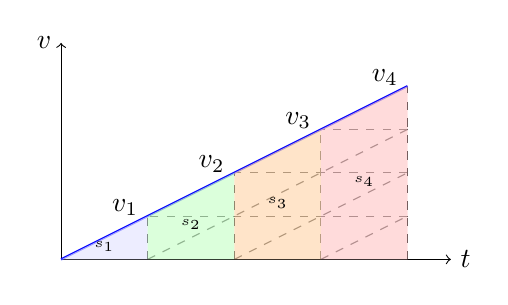
\begin{tikzpicture}[scale=1.1]
    % 坐标轴
    \draw[->] (0,0) -- (0,2.5) node[left] {$v$};
    \draw[->] (0,0) -- (4.5,0) node[right] {$t$};
    % 等时间间隔
    \foreach \i in {1,2,3,4}
    \draw[dashed] (\i,0) -- (\i,\i*0.5);
    \foreach \i in {1,2,3}
    \draw[dashed] (4,\i*0.5) -- (\i,\i*0.5);
    \foreach \i in {1,2,3}
    \draw[dashed] (\i,0) -- (4,2-\i*0.5);
    % 匀加速直线
    \draw[thick,blue] (0,0) -- (4,2);
    % 速度标记
    \foreach \i/\v in {0/1,1/2,2/3,3/4}
    \node[left] at (\i+1,\i*0.5+0.6) {$v_{\the\numexpr\i+1}$};
    \foreach \i/\col in {0/blue!10, 1/green!20, 2/orange!30, 3/red!20} {
      \fill[\col,opacity=0.7] (\i,0) -- (\i+1,0) -- (\i+1,\i*0.5+0.5) -- (\i,\i*0.5);
      \node at (\i+0.5,\i*0.25+0.15) {\tiny $s_{\the\numexpr\i+1}$};
    }
  \end{tikzpicture}
\end{minipage}
\hfill
\begin{minipage}{0.48\columnwidth}
  \centering
  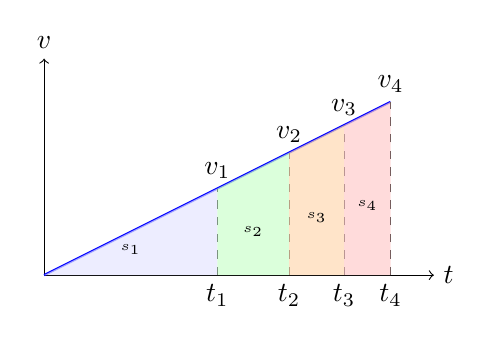
\begin{tikzpicture}[scale=1.1]
    % 坐标轴
    \draw[->] (0,0) -- (0,2.5) node[above] {$v$};
    \draw[->] (0,0) -- (4.5,0) node[right] {$t$};
    % 匀加速直线
    \draw[thick,blue] (0,0) -- (4,2);
    % 等位移间隔
    \foreach \i in {1,2,3,4}
    \draw[dashed] ({2*sqrt(\i)},0) -- ({2*sqrt(\i)},{sqrt(\i)});
    % 时间标记
    \node[below] at (2,0) {$t_1$};
    \node[below] at ({2*sqrt(2)},0) {$t_2$};
    \node[below] at ({2*sqrt(3)},0) {$t_3$};
    \node[below] at ({2*sqrt(4)},0) {$t_4$};
    % % 位移阴影
    \foreach \i/\col in {1/blue!10, 2/green!20, 3/orange!30, 4/red!20} {
      \fill[\col,opacity=0.7] ({2*sqrt(\i-1)},0) -- ({2*sqrt(\i)},0) -- ({2*sqrt(\i)},{sqrt(\i)}) -- ({2*sqrt(\i-1)},{sqrt(\i-1)});
      \node at ({(sqrt(\i)+sqrt(\i-1))},{sqrt(\i)*0.5-0.2}) {\tiny $s_{\the\numexpr\i}$};
    }
    \foreach \i in {1,2,3,4}
    \node[above] at ({2*sqrt(\i)},{sqrt(\i)}) {$v_{\the\numexpr\i}$};
  \end{tikzpicture}
\end{minipage}

\begin{tabularx}{\columnwidth}{XX}
  \rowcolor{blue!30}
  \multicolumn{2}{l}{\parbox[c][2.5\ht\strutbox][c]{0.9\columnwidth}{\Large 力学}} \\
  重力&$G=mg$\\
  弹簧弹力&$F=k\Delta x$\\
  滑动摩擦力&$F=\mu N$\\
  合力范围&$|F_1-F_2|\le F \le |F_1+F_2|$\\
\end{tabularx}
\hfill
\begin{minipage}{0.8\columnwidth}
  \centering
  \begin{tikzpicture}[scale=1.2]
    % 竖直位置
    \def\yA{2.5}
    \def\yB{1.2}
    \def\yC{0}
    % 弹簧长度
    \def\L{2.5}
    \def\stretch{1.0}
    \def\compress{1.0}
    % 左端对齐的x坐标
    \def\xL{0.5}
    % 右端x坐标
    \def\xA{\xL+\L}
    \def\xB{\xL+\L+\stretch}
    \def\xC{\xL+\L-\compress}
    % 原长弹簧
    \draw[thick,decorate,decoration={coil,aspect=0.5,segment length=3mm,amplitude=2mm}] (\xL,\yA) -- (\xA,\yA);
    \filldraw[gray] (\xL,\yA) circle (0.09);
    \filldraw[gray] (\xA,\yA) circle (0.09);
    \node[above] at ({(\xL+\xA)/2},\yA+0.18) {\small 原长 $l_0$};
    % 拉伸弹簧
    \draw[thick,decorate,decoration={coil,aspect=0.5,segment length=3mm,amplitude=2mm}] (\xL,\yB) -- (\xB,\yB);
    \filldraw[gray] (\xL,\yB) circle (0.09);
    \filldraw[gray] (\xB,\yB) circle (0.09);
    % 拉力箭头
    \draw[->,red,thick] (\xB,\yB) -- ++(0.7,0) node[right] {\small $F_\text{拉}$};
    \node[above] at ({(\xL+\xB)/2},\yB+0.18) {\small 拉伸 $l_0+\Delta l$};
    % 压缩弹簧
    \draw[thick,decorate,decoration={coil,aspect=0.5,segment length=3mm,amplitude=2mm}] (\xL,\yC) -- (\xC,\yC);
    \filldraw[gray] (\xL,\yC) circle (0.09);
    \filldraw[gray] (\xC,\yC) circle (0.09);
    % 压力箭头
    \draw[<-,blue,thick] (\xC,\yC) -- ++ (0.7,0) node[right] {\small $F_\text{压}$};
    \node[above] at ({(\xL+\xC)/2},\yC+0.18) {\small 压缩 $l_0-\Delta l$};
    % 末端比较连线
    \draw[thick,gray!60!black,dashed] (\xA,\yA) -- (\xA,\yC);
    \draw[thick,gray!60!black,dashed] (\xB,\yA) -- (\xB,\yC);
    \draw[thick,gray!60!black,dashed] (\xC,\yA) -- (\xC,\yC);
  \end{tikzpicture}
\end{minipage}
\hfill
\begin{minipage}
  {0.45\columnwidth}
  \centering
  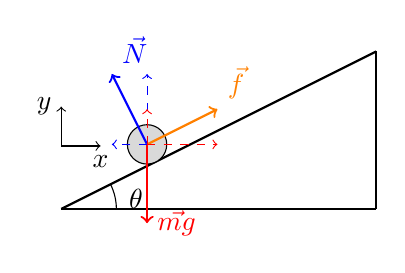
\begin{tikzpicture}[scale=1]
    \draw[thick] (0,0) -- (4,0);
    \draw[thick] (0,0) -- (4,2);
    \draw[thick] (4,0) -- (4,2);
    \filldraw[fill=gray!30] (1.09,0.82) circle (0.25);
    \draw[->,thick,red] (1.09,0.82) -- ++(0,-1) node[right] {$\vec{mg}$};
    \draw[->,thick,blue] (1.09,0.82) -- ++(-0.447,0.894) node[above right] {$\vec{N}$};
    \draw[->,thick,orange] (1.09,0.82) -- ++(0.894,0.447) node[above right] {$\vec{f}$};
    \draw[->] (0,0.8) -- ++(0,0.5) node[left] {$y$};
    \draw[->] (0,0.8) -- ++(0.5,0) node[below] {$x$};
    \draw[->,dashed, blue] (1.09,0.82) -- ++(0,0.894) node[left] {};
    \draw[->,dashed, blue] (1.09,0.82) -- ++(-0.447,0) node[below] {};
    \draw[->,dashed, red] (1.09,0.82) -- ++(0.894,0) node[below right] {};
    \draw[->,dashed, red] (1.09,0.82) -- ++(0,0.447) node[left] {};
    \draw (0.7,0) arc (0:26.565:0.7);
    \node at (0.95,0.13) {$\theta$};
  \end{tikzpicture}\\
  水平和竖直方向分解
\end{minipage}
\hfill
\begin{minipage}{0.45\columnwidth}
  \centering
  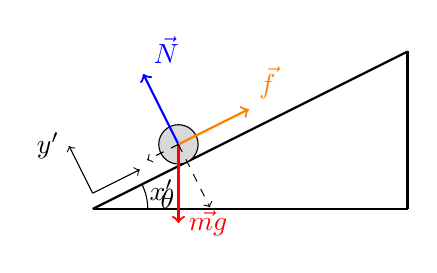
\begin{tikzpicture}[scale=1]
    \draw[thick] (0,0) -- (4,0);
    \draw[thick] (0,0) -- (4,2);
    \draw[thick] (4,0) -- (4,2);
    \filldraw[fill=gray!30] (1.09,0.82) circle (0.25);
    \draw[->,thick,red] (1.09,0.82) -- ++(0,-1) node[right] {$\vec{mg}$};
    \draw[->,thick,blue] (1.09,0.82) -- ++(-0.447,0.894) node[above right] {$\vec{N}$};
    \draw[->,thick,orange] (1.09,0.82) -- ++(0.894,0.447) node[above right] {$\vec{f}$};
    \draw[->,dashed] (1.09,0.82) -- ++(-0.4,-0.2) node[above right] {};
    \draw[->,dashed] (1.09,0.82) -- ++(0.4,-0.8) node[left] {};
    \draw[->] (0,0.2) -- ++(0.6,0.3) node[below right] {$x'$};
    \draw[->] (0,0.2) -- ++(-0.3,0.6) node[left] {$y'$};
    \draw (0.7,0) arc (0:26.565:0.7);
    \node at (0.95,0.13) {$\theta$};
  \end{tikzpicture}\\
  沿斜面和垂直斜面分解
\end{minipage}

\begin{tabularx}{\columnwidth}{XX}
  \rowcolor{blue!30}
  \multicolumn{2}{l}{\parbox[c][2.5\ht\strutbox][c]{0.9\columnwidth}{\Large 平抛运动}} \\
  水平位移&$x=v_0t$\\
  竖直位移&$y=\frac{1}{2}gt^2$\\
  竖直速度&$v_y=gt=v_0\tan\theta$\\
  速度大小&$v=\sqrt{v_0^2+g^2t^2}=\frac{v_0}{\cos\theta}$\\
  速度方向&$\tan\theta=\frac{gt}{v_0}=\frac{2y}{x}$\\
  运动时间&$t=\sqrt{\frac{2y}{g}}$\\
\end{tabularx}
\notice{
  平抛运动落在斜面上，速度方向正好垂直于斜面。\\
  此时可以利用如下的比例关系求解：\\
  $h$为抛出高度，$x$为水平位移，$y$为竖直位移。\\
  $\theta$为斜面倾角，$v_0$为抛出速度，$v_y$为竖直速度。\\
  \[\tan\theta=\frac{h-y}{x}=\frac{x}{2y}=\frac{v_0}{v_y}\]
}
\begin{minipage}{0.48\columnwidth}
  \centering
  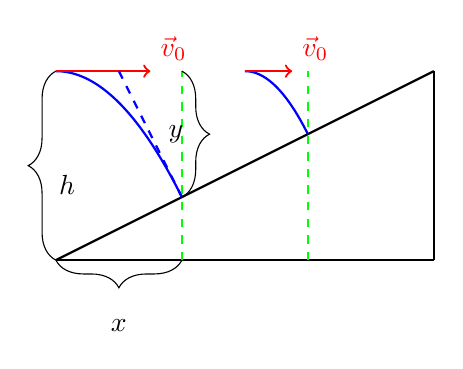
\begin{tikzpicture}[scale=1.2]
    \draw[thick] (0,0) -- (4,0);
    \draw[thick] (0,0) -- (4,2);
    \draw[thick] (4,0) -- (4,2);
    \draw[thick,blue,domain=0:4/3,samples=100] plot (\x,{2-0.75*\x^2});
    \draw[->,red,thick] (0,2) -- (1,2) node[above right] {$\vec{v}_0$};
    \draw[dashed, thick, green] (4/3,0) -- (4/3,2);
    \draw[dashed, thick, blue, domain=(2/3):(4/3), samples=100] plot (\x, {10/3-2*\x});

    \draw[thick,blue,domain=2:8/3,samples=100] plot (\x,{2-1.5*(\x-2)^2});
    \draw[->,red,thick] (2,2) -- (2.5,2) node[above right] {$\vec{v}_0$};
    \draw[dashed, thick, green] (8/3,0) -- (8/3,2);

    \draw [decorate,decoration={brace,mirror,amplitude=10pt}] (0,0) -- (4/3,0) node[midway, yshift=-18pt, below] {$x$};
    \draw [decorate,decoration={brace,amplitude=10pt}] (4/3,2) -- (4/3,2/3) node[midway, xshift=4pt, left] {$y$};
    \draw [decorate,decoration={brace,amplitude=10pt}] (0,0) -- (0,2) node[midway, xshift=4pt, below] {$h$};
  \end{tikzpicture}
\end{minipage}

\notice{
  从斜面上出发的平抛运动，落回点也在斜面上。\\
  设斜面倾角为$\theta$，水平位移为$x$，竖直位移为$y$。\\
  一定有
  \[\tan\theta=\frac{y}{x}\]
}
\begin{minipage}{0.48\columnwidth}
  \centering
  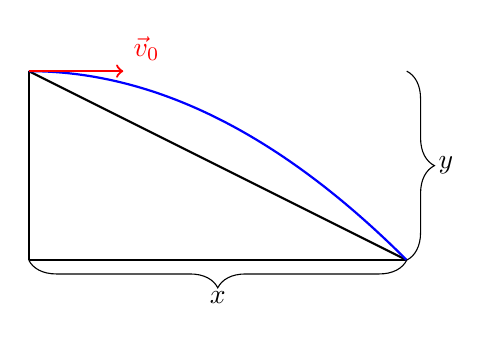
\begin{tikzpicture}[scale=1.2]
    \draw[thick] (0,0) -- (4,0);
    \draw[thick] (0,0) -- (0,2);
    \draw[thick] (0,2) -- (4,0);
    \draw[thick, blue, domain=0:4, samples=100] plot (\x,{2-1/8*\x^2});
    \draw[->,red,thick] (0,2) -- (1,2) node[above right] {$\vec{v}_0$};
    \draw [decorate,decoration={brace,amplitude=10pt}] (4,2) -- (4,0) node[midway, xshift=8pt, right] {$y$};
    \draw [decorate,decoration={brace,mirror,amplitude=10pt}] (0,0) -- (4,0) node[midway, yshift=-8pt, below] {$x$};
  \end{tikzpicture}
\end{minipage}

\notice{
  通过固定水平位移时，合速度最小时，水平与竖直方向速度相等。
  推导过程：
  \[v^2=v_0^2+v_y^2\]
  代入
  \[v_y^2=(at)^2=\frac{a^2x^2}{v_0^2}\]
  得
  \[v^2=v_0^2+\frac{a^2x^2}{v_0^2}\ge 2ax \]
  当且仅当$v_0=\sqrt{ax}$时等号成立，并且此时有$v_0=v_y$。即合速度存在最小值。
}

% \notice{
%     \begin{itemize}
%         \item 平抛运动经过片固定水平位移，合速度最小为$\sqrt2v_0$，此时速度夹角为$45^\circ$。
%         \item 平抛运动落在斜面上速度与斜面垂直时
%         \item
%     \end{itemize}
% }
\end{document}
